%!TEX root = ../../../thesis.tex

\chapter{Supplementary Figures}\label{app:network_analysis}

This appendix contains figures supplementing \Fref{chap:analysis}. Note that the full set of goodness-of-fit plots for all data series is available online at the \SMGR. 

\section{Goodness-of-fit Plots for \Fref{sec:analysis_results}}

\begin{figure}[!htbp]
\begin{center}%
  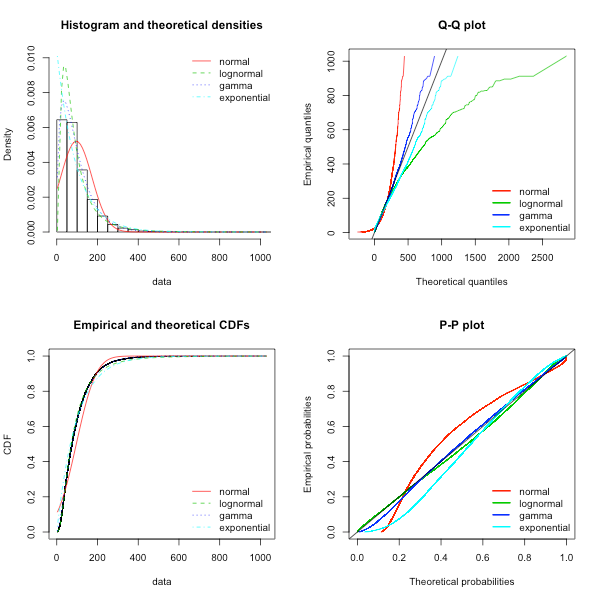
\includegraphics[width=0.9\textwidth]{path_length/physical_edge_length_histogram_cummulative_motion22.png}
\end{center}%
\caption[Goodness-of-fit plots - Path lengths]{Goodness-of-fit plots of fitting the empirical path length distribution of \series{22} comparing various common theoretical distributions.}
\label{fig:sup::path_lengths_goodness}
\end{figure}

\begin{figure}[!htbp]
\begin{center}%
  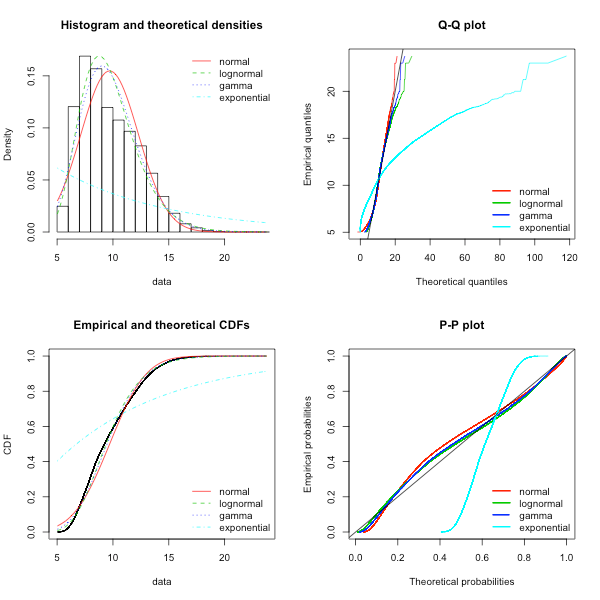
\includegraphics[width=\textwidth]{path_width/physical_edge_width_histogram_cummulative_motion35.png}
\end{center}%
\caption[Goodness-of-fit plots - Path widths]{Goodness-of-fit plots of fitting the empirical average path widths distribution of \series{22} comparing various common theoretical distributions.}
\label{fig:sup::path_widths_goodness}
\end{figure}

\begin{figure}[!htbp]
\begin{center}%
  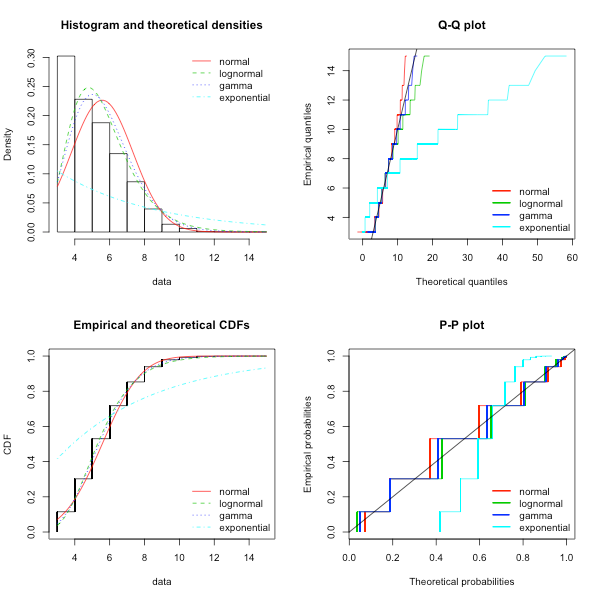
\includegraphics[width=\textwidth]{face_degree/dual_node_degree_histogram_cummulative_motion35.png}
\end{center}%
\caption[Goodness-of-fit plots - Face degrees]{Goodness-of-fit plots of fitting the empirical face degree distribution of \series{22} comparing various common theoretical distributions. Since the degree distribution is a discrete distribution while the fitted distributions are continuous, we obtain the observed steps. We did not look towards fitting discrete distributions.}
\label{fig:sup::face_degree_goodness}
\end{figure}

\begin{figure}[!htbp]
\begin{center}%
  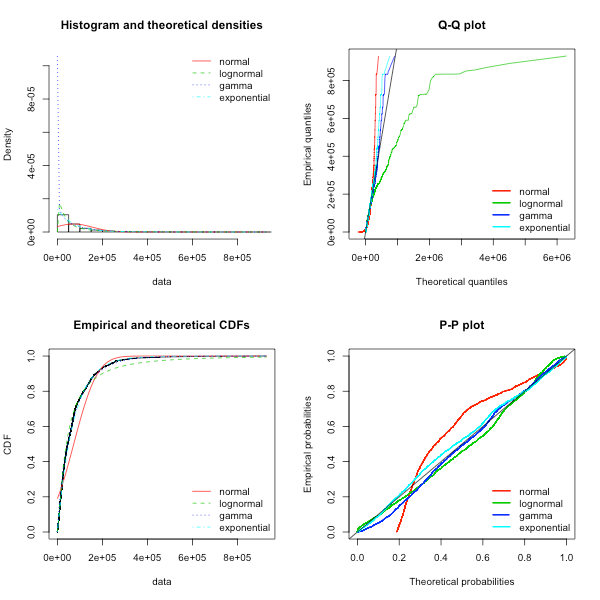
\includegraphics[width=\textwidth]{face_area/face_area_histogram_cummulative_motion35.png}
\end{center}%
\caption[Goodness-of-fit plots - Face area]{Goodness-of-fit plots of fitting the empirical face area distribution of \series{22} comparing various common theoretical distributions.}
\label{fig:sup::face_area_goodness}
\end{figure}

\begin{figure}[!htbp]
\begin{center}%
  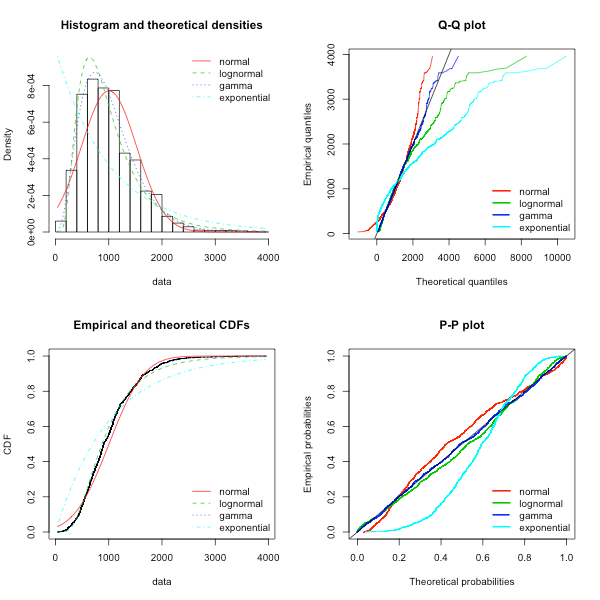
\includegraphics[width=\textwidth]{face_length/face_length_histogram_cummulative_motion35.png}
\end{center}%
\caption[Goodness-of-fit plots - Face circumference]{Goodness-of-fit plots of fitting the empirical face circumference distribution of \series{22} comparing various common theoretical distributions.}
\label{fig:sup::face_length_goodness}
\end{figure}

\section{Addititonal Illustrations for \Fref{sec:cut_properties}}

\vfill
\begin{figure}[!htbp]
\begin{center}%
  \includegraphics[width=\textwidth]{cuts/physarum_sequence_4.JPG}
\end{center}%
\caption[Horizontal and vertical cuts illustrated]{After a while the growing front has escaped the area of observation leaving behind its supporting vein network. We consider the network within a predefined region of interest (dotted rectangle). We subdivide this region of interest by defining 100 equidistant vertical and horizontal lines. The intersection of the vein network with these lines define cuts. Horizontal cuts proceed from top to bottom, \ie perpendicular to the growth direction. Vertical cuts proceed from left to right, \ie in growth direction. Solid lines show one cut of each type.}
\label{fig:sup::physarum_roi}
\end{figure}
\vfill
\begin{figure}[!htbp]
\begin{center}%
  \includegraphics[width=\textwidth]{cuts/physarum_sequence_2.JPG}
\end{center}%
\caption[Detail of the apical zone]{\P advancing its growing front and expanding along the positive x-axis. The front itself is approximately paralell to the y-axis, \ie perpendicular to the direction of growth.}
\label{fig:sup::physarum_expanding}
\end{figure}
\vfill

